\chapter{O que dizem os números}
\markboth{Módulo 1}{}

\vspace*{-1cm}

\section*{Habilidades do SAEB}


\begin{itemize}
  \item Escrever números racionais (naturais de até 6 ordens, representação
fracionária ou decimal finita até a ordem dos milésimos) em sua
representação por algarismos ou em língua materna ou associar o registro
numérico ao registro em língua materna.

  \item Identificar a ordem ocupada por um algarismo ou seu valor posicional
(ou valor relativo) em um número natural de até 6 ordens.

  \item Comparar ou ordenar números racionais (naturais de até 6 ordens,
representação fracionária ou decimal finita até a ordem dos milésimos),
com ou sem suporte da reta numérica.

  \item Compor ou decompor números naturais de até 6 ordens na forma aditiva,
ou em suas ordens, ou em adições e multiplicações.

  \item Comparar diferentes sentenças de adições ou de subtrações de dois
números naturais.

  \item Determinar o número desconhecido que torna verdadeira uma igualdade
que envolve as operações fundamentais com números naturais de até 6
ordens.
\end{itemize}


\subsection{Habilidades da BNCC}

\begin{itemize}
\item EF03MA01, EF03MA04.
\end{itemize}

\conteudo{
Valor absoluto é o valor numérico do próprio algarismo, e o valor posicional, também conhecido como valor relativo, refere-se ao lugar que o algarismo ocupa no número, considerando a classe e a ordem. 
 
Exemplo.

No número 2.146, o algarismo 1 possui valor posicional ou
relativo igual a 100, pois ocupa a classe da centena, na 3ª ordem. 
Sendo assim, 1 x 100 = 100.

Com essas informações, é possível decompor o número 2.146, de acordo com a posição que cada algarismo ocupa no número: 2.146 = 2 x 1.000 + 1 x 100 + 4 x 10 + 6.

\vspace{1ex}
\noindent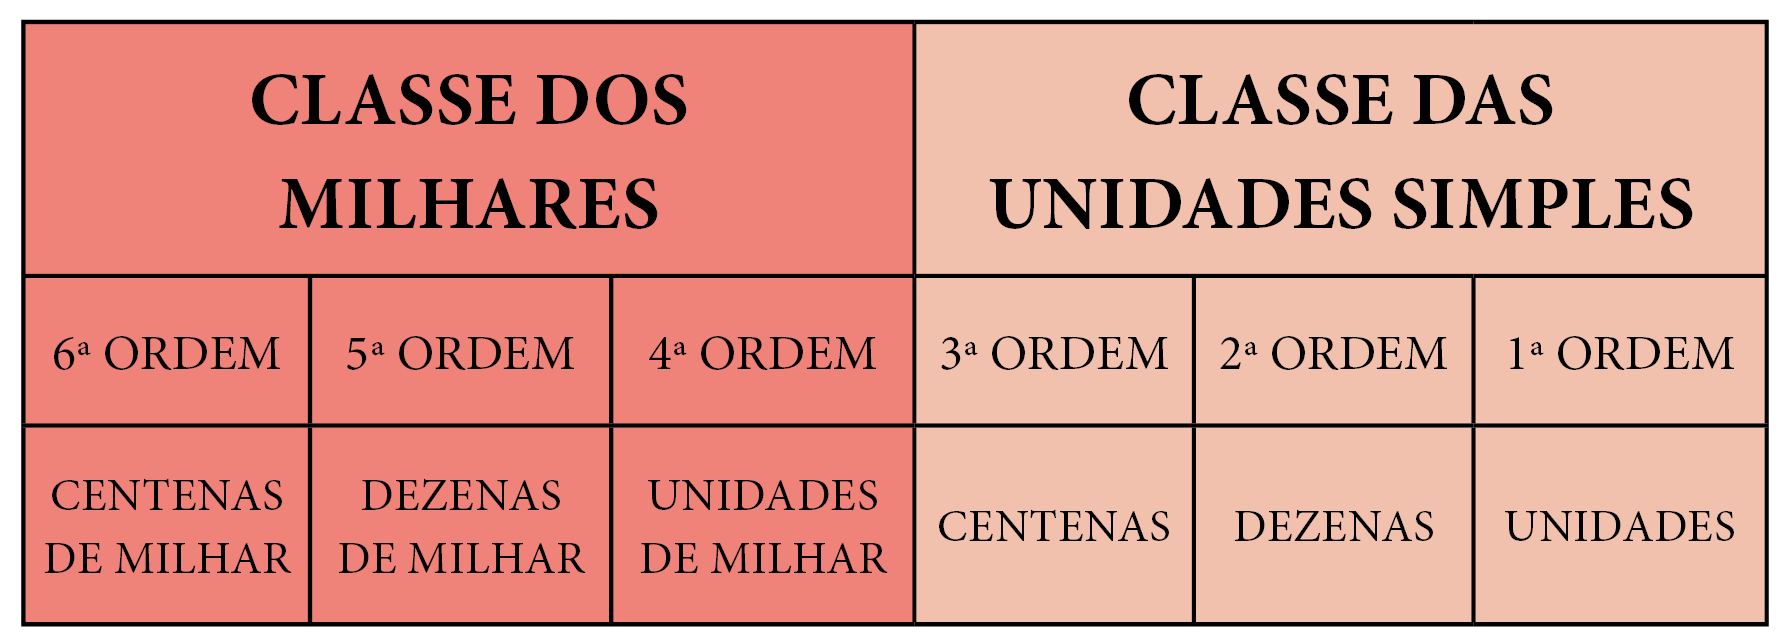
\includegraphics[width=\textwidth]{./media/image1.png}
}

\section*{Atividades}

\num{1} Vilma encontrou um pedaço de papel na sua bolsa. Nele, estava escrito o número a seguir:

\begin{figure}[htpb!]
\centering
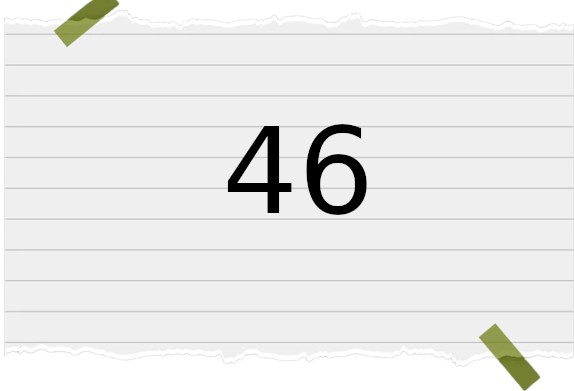
\includegraphics[width=.5\textwidth]{./media/image2.png}
\end{figure}

\pagebreak

\begin{escolha}
\item  Escreva o número 46 por extenso.
\reduline{Quarenta e seis.\hfill}
\linhas{1}

\item Calcule quantos grupos de 10 unidades é possível formar com o número 46.
\reduline{É possível formar 4 grupos de 10 unidades, e restam 6 que não são suficientes para formar outro grupo completo. Portanto, podemos expressar isso como 46 = 4 x 10 + 6\hfill}
\end{escolha}

\num{2} Arnaldo contou suas figurinhas. Com elas, ele montou 8 grupos com 10 figurinhas cada, e ainda adicionou mais quatro figurinhas ao total.

\begin{figure}[htpb!]
\centering
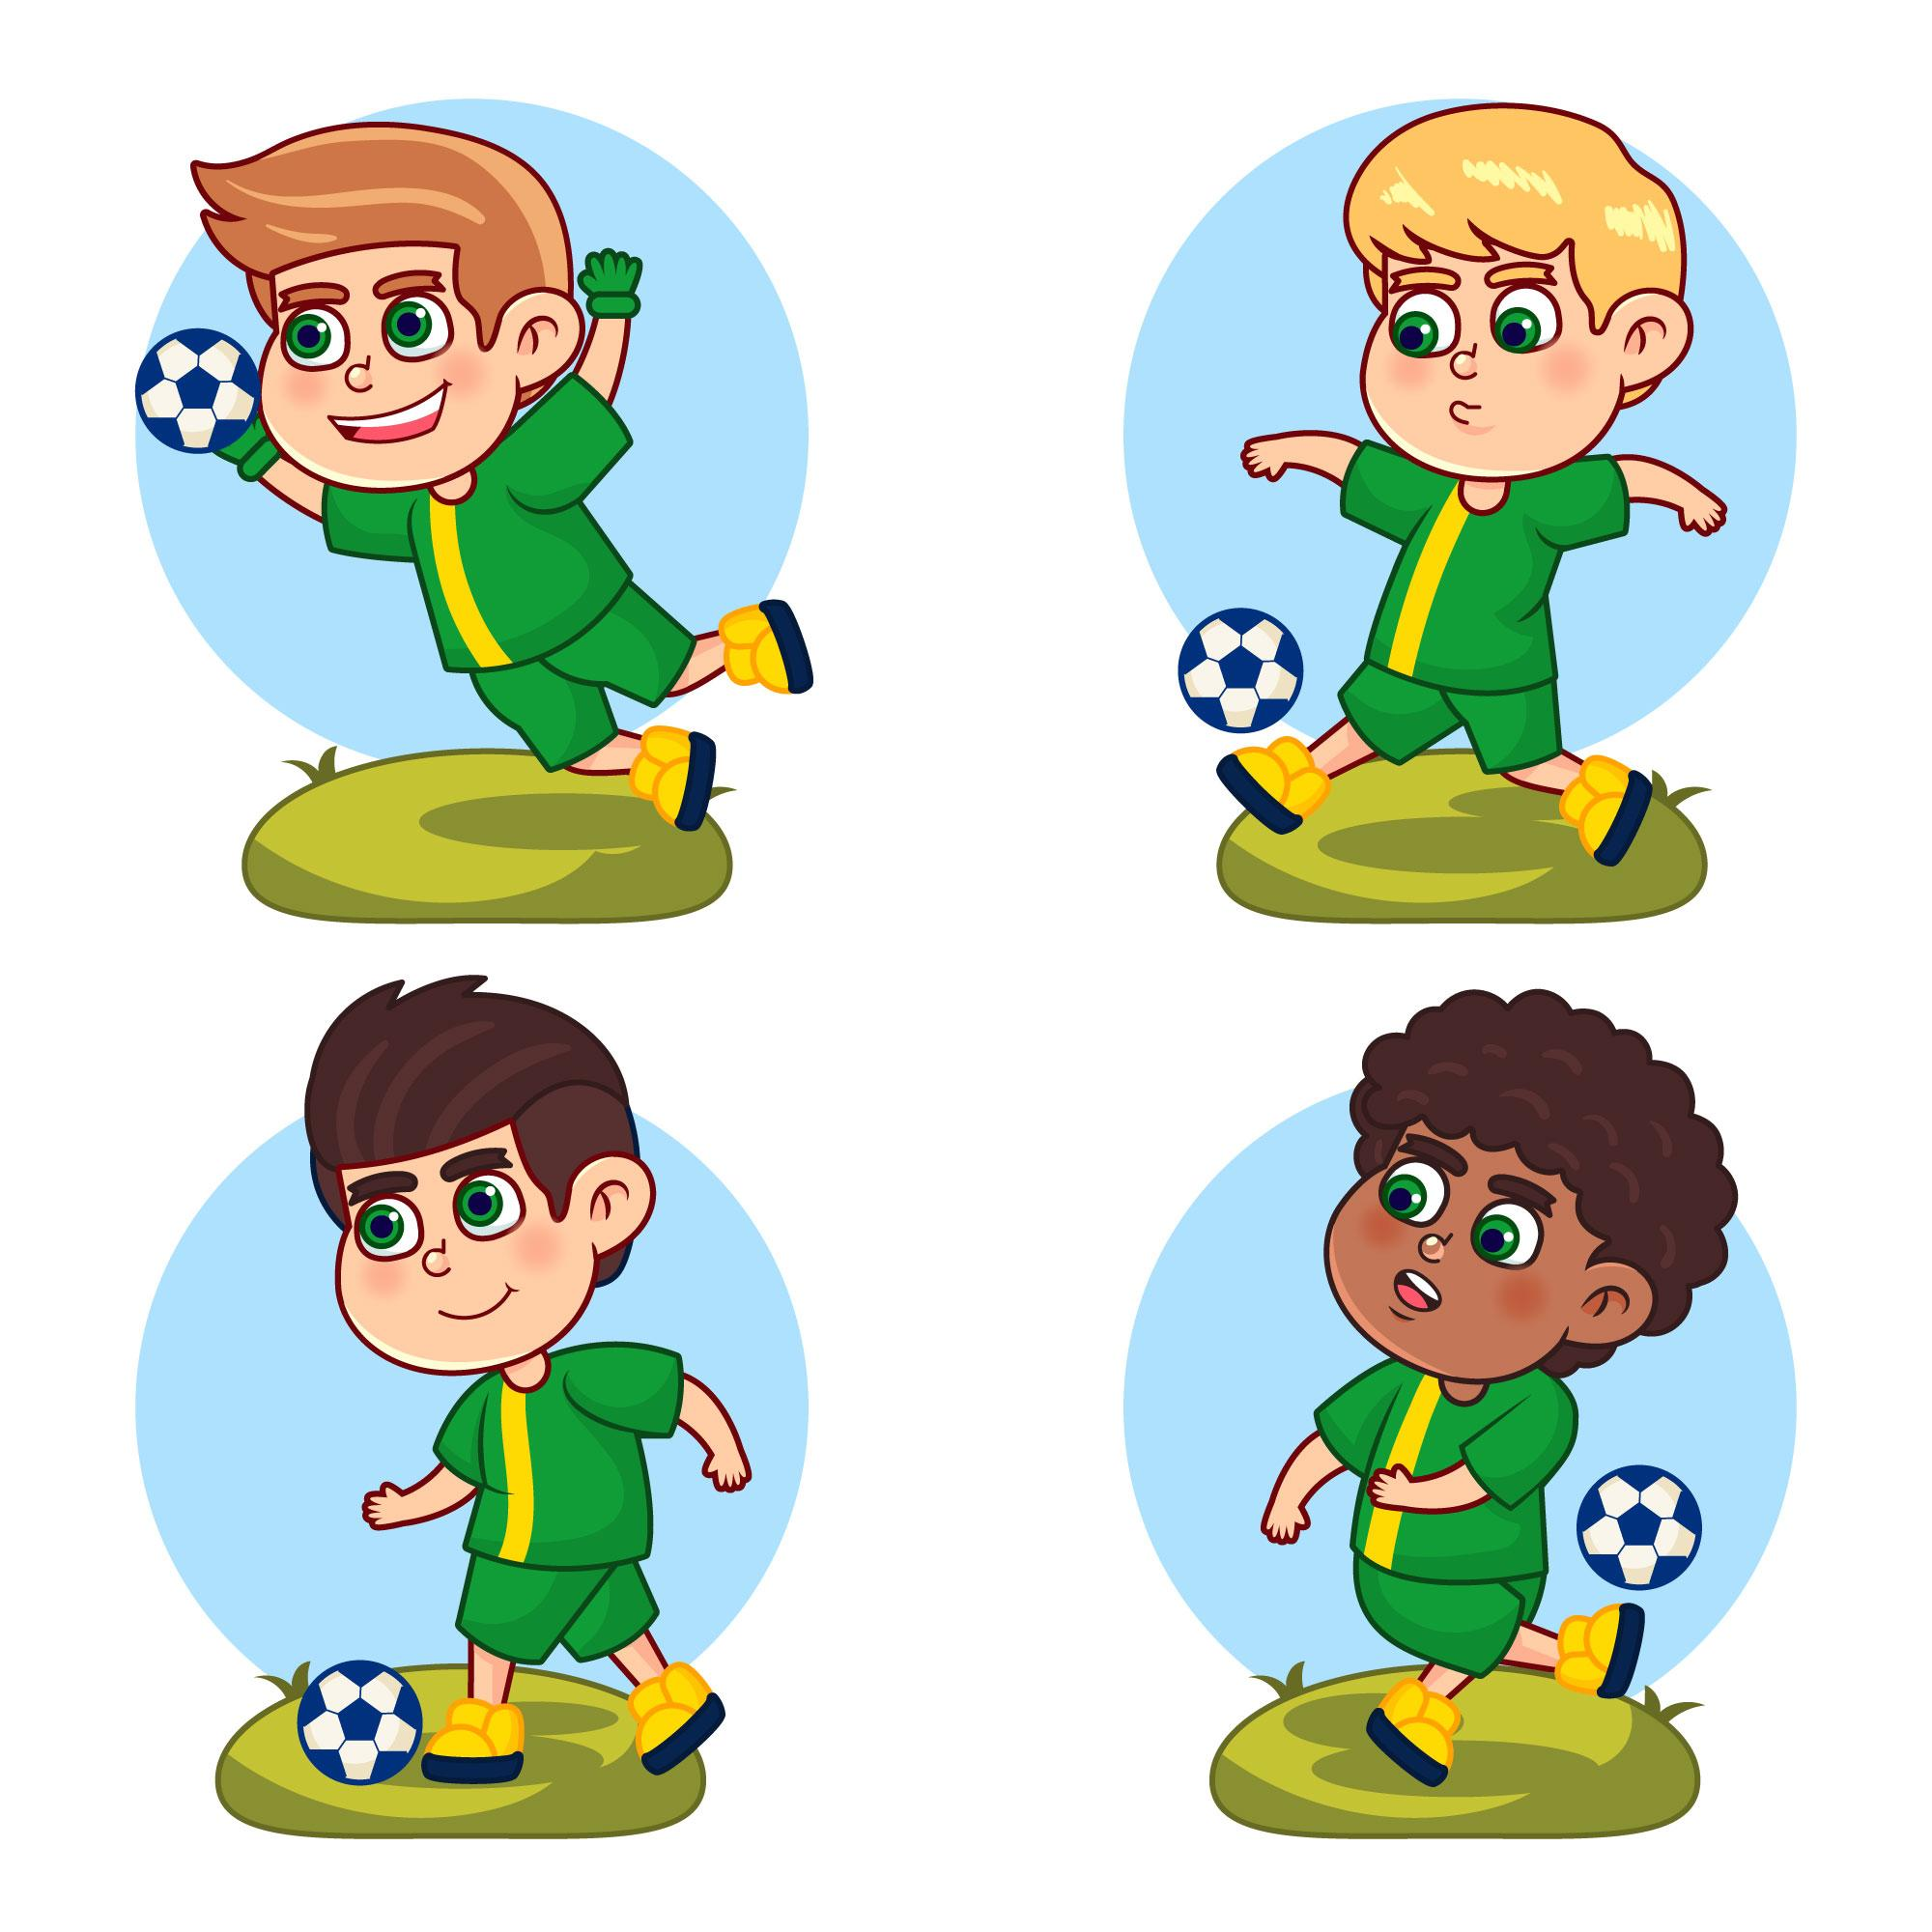
\includegraphics[width=.6\textwidth]{./media/image2a.jpg}
\end{figure}

\begin{escolha}
\item
  Calcule o número de figurinhas que Arnaldo possui.\\
\reduline{8 x 10 + 4 = 84\hfill}

\item  Escreva o número de figurinha que Arnaldo possui por extenso.\\
\reduline{Oitenta e quatro.\hfill}
\end{escolha}

\num{3} Treine sua criatividade, escrevendo:

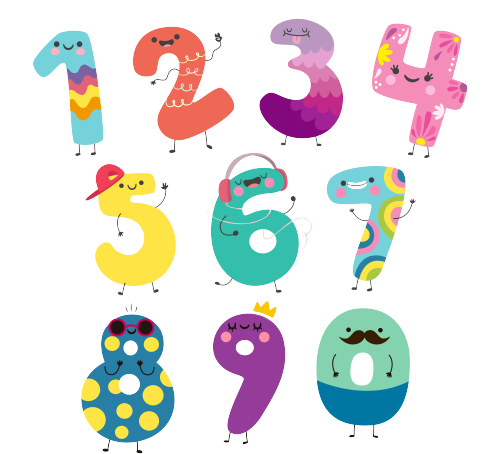
\includegraphics[width=\textwidth]{./media/image4a.png}

\begin{escolha}
\item Um número formado por três algarismos iguais.\\
\reduline{Resposta pessoal. Exemplo: 222.\hfill}

\item Um número formado por três algarismos no qual o 0 (zero) seja o terceiro algarismo.\\
\reduline{Resposta pessoal. Exemplo: 390.\hfill}

\item Um número formado por três algarismos diferentes.\\
\reduline{Resposta pessoal. Exemplo: 159.\hfill}

\item Um número com mais de três algarismos.\\
\reduline{Resposta pessoal. Exemplo: 1.477.\hfill}

\item Mostre os números que você criou para um colega e veja os números que ele criou.
\end{escolha}

\num{4} Escreva o número em algarismos ao lado de cada item e, em seguida, decomponha o número de acordo com o modelo.

\begin{myquote}
\begin{center}
\textbf{Cento e vinte e sete:} \textbf{127 = 100 + 20 + 7.}
\end{center}
\end{myquote}

\begin{escolha}
\item Trezentos e cinquenta e quatro.
\reduline{354 = 300 + 50 + 4.\hfill}

\item Duzentos e vinte e oito.
\reduline{228 = 200 + 20 + 8.\hfill}

\item Quatrocentos e setenta e seis.
\reduline{476 = 400 + 70 + 6.\hfill}
\end{escolha}

\num{5} Complete o quadro de acordo com a orientação.\bigskip

\noindent\begin{tabular}{llll}
\hline
\vspace{1.5em}
\begin{tabular}[c]{@{}l@{}}\textbf{Número escrito}\\ \textbf{por extenso}\end{tabular} & \begin{tabular}[c]{@{}l@{}}\textbf{Número escrito}\\ \textbf{em algarismos}\end{tabular} & \textbf{Número decomposto} \\ 
\hline
\vspace{1em}
Quinhentos e vinte e seis & \rosa{526} & \rosa{500} + 20 + 6 \\
\hline
\vspace{1em}
\rosa{Quatrocentos e trinta e cinco} & 435 & \rosa{400} + 30 + 5 \\
\hline
\vspace{1em}
\rosa{Oitocentos e trinta e dois} & \rosa{832} & 800 + 30 + 2 \\
\hline
\vspace{1em}
\rosa{Setecentos e vinte e nove} & \rosa{729} & 700 + 20 + 9 \\ 
\hline
\vspace{1em}
\rosa{Seiscentos e quarenta e um} & 641 & \rosa{600 + 40 + 1} \\ 
\hline
\end{tabular}

\pagebreak

\num{6} Durante a aula, Gabriel aprendeu a montar números utilizando o
material dourado. Ele montou o número abaixo:

%Produzir uma imagem semelhante a essa abaixo com 5 barras de 10 cubinhos cada e 9 cubinhos separados. Deixar a figura melhor apresentável e, se possível, numa cor parecida com o dourado.
\vspace{1.5em}

\begin{figure}[htpb!]
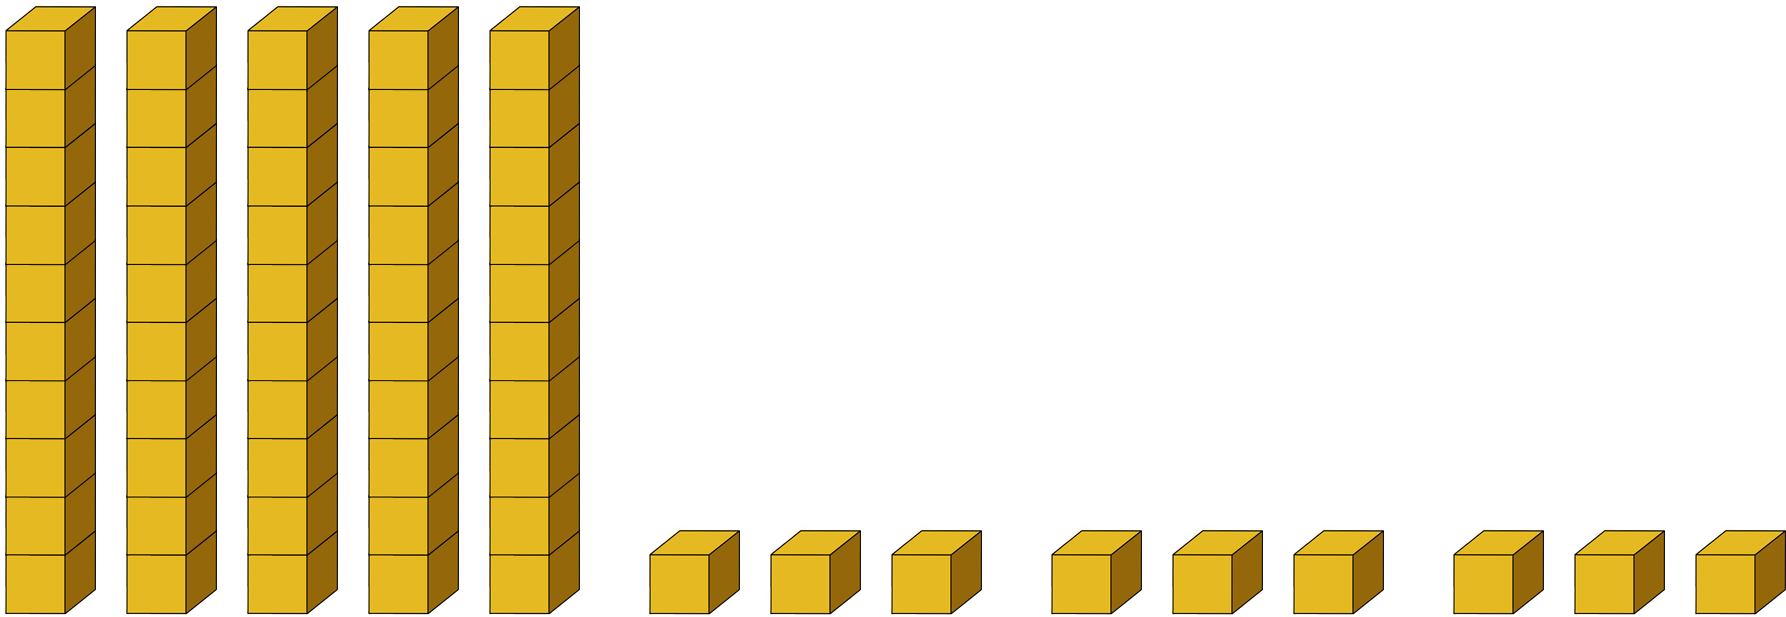
\includegraphics[width=\textwidth]{./media/image3.png}
\end{figure}
\vspace{1.5em}

\begin{escolha}
\item Qual é o número de cubos dourados representado na figura?
\reduline{Na figura, o número de cubos dourado é 59.\hfill}
\linhas{1}

\item Como o número montado por Gabriel pode ser decomposto?
\reduline{50 x 10 + 9 = 59.\hfill}
\linhas{1}
\end{escolha}

\num{7} Complete as informações abaixo de acordo com o que se pede. 

\begin{escolha}
\item
  Fernando tem 4 dezenas de lápis mais 2 unidades.

\begin{longtable}[]{@{}lll@{}}
\toprule
\textbf{Dezena} & \textbf{Unidade}\tabularnewline
\midrule
\endhead
&\tabularnewline
\bottomrule
\end{longtable}


Total de lápis que Fernando possui:
\reduline{4 x 10 + 2 = 42. Quarenta e dois lápis.\hfill}

\item Thiago tem 8 dezenas de bolinhas de gude mais 5 unidades.

\begin{longtable}[]{@{}lll@{}}
\toprule
\textbf{Dezena} & \textbf{Unidade}\tabularnewline
\midrule
\endhead
&\tabularnewline
\bottomrule
\end{longtable}

Total de bolinhas de gude que Thiago possui:
\reduline{8 x 10 + 5 = 85. Oitenta e cinco bolinhas de gude.\hfill}
\end{escolha}

\num{8} Realize a decomposição dos números indicados em cada item.

\begin{escolha}
\item 56: \reduline{5 x 10 + 6 = 56.\hfill}

\item 73: \reduline{7 x 10 + 3 = 73.\hfill}

\item 94: \reduline{9 x 10 + 4 = 94.\hfill}

\item 14: \reduline{1 x 10 + 4 = 14.\hfill}

\item 81: \reduline{8 x 10 + 1 = 81.\hfill}

\item 158: \reduline{1 x 100 + 5 x 10 + 8 = 158.\hfill}

\item 649: \reduline{6 x 100 + 4 x 10 + 9 = 649.\hfill}

\item 784: \reduline{7 x 100 + 8 x 10 + 4 = 784.\hfill}

\item 925: \reduline{9 x 100 + 2 x 10 + 5 = 925.\hfill}

\item 1.247: \reduline{1 x 1.000 + 2 x 200 + 4 x 10 + 7 = 1.247.\hfill}
\end{escolha}

\pagebreak

\num{9} Richard encontrou as seguintes peças de um material dourado:

\begin{figure}[htpb!]
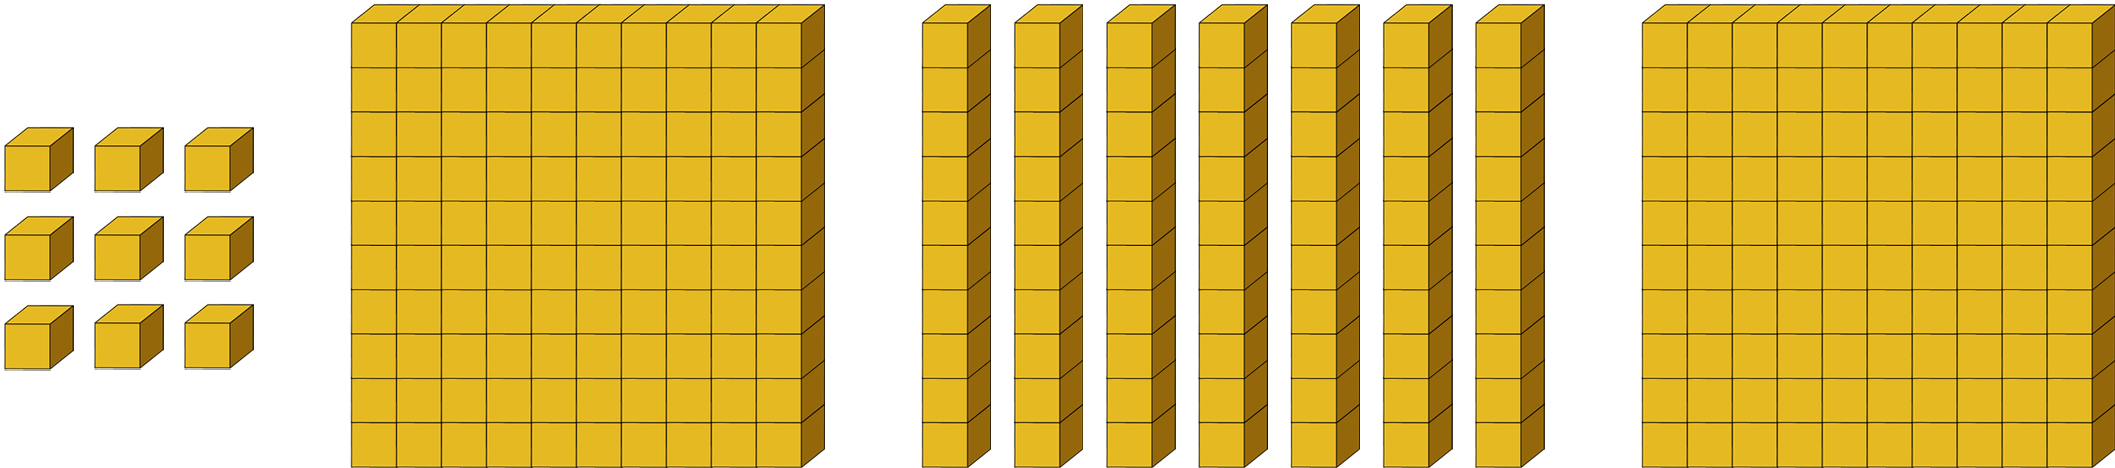
\includegraphics[width=\textwidth]{./media/image4.png}
\end{figure}

Somando todas as peças, qual o maior número que Richard pode representar? 
\reduline{2 x 100 + 7 x 10 + 9 = 279.\hfill}
\linhas{3}

Após encontrar o número, escreva-o por extenso.
\reduline{Duzentos e setenta e nove.\hfill}
\linhas{1}

\num{10} Monte os números compostos e escreva-os nos locais correspondentes.

\begin{escolha}
\item 5 centenas e 4 unidades:
\reduline{504.\hfill}

\item 7 dezenas e 2 unidades:
\reduline{2.\hfill}

\item 9 centenas, 5 dezenas e 6 unidades:
\reduline{956.\hfill}

\item 2 centenas, 6 dezenas e 3 unidades:
\reduline{263.\hfill}

\item 4 dezenas e 8 unidades
\reduline{48.\hfill}

\item 1 unidade de milhar, 7 centenas, 1 dezena e 9 unidades
\reduline{1.719.\hfill}

\end{escolha}


\num{11} Leia o enunciado e responda ao que se pede. 

\vspace{1em}

\begin{figure}[htpb!]
\centering
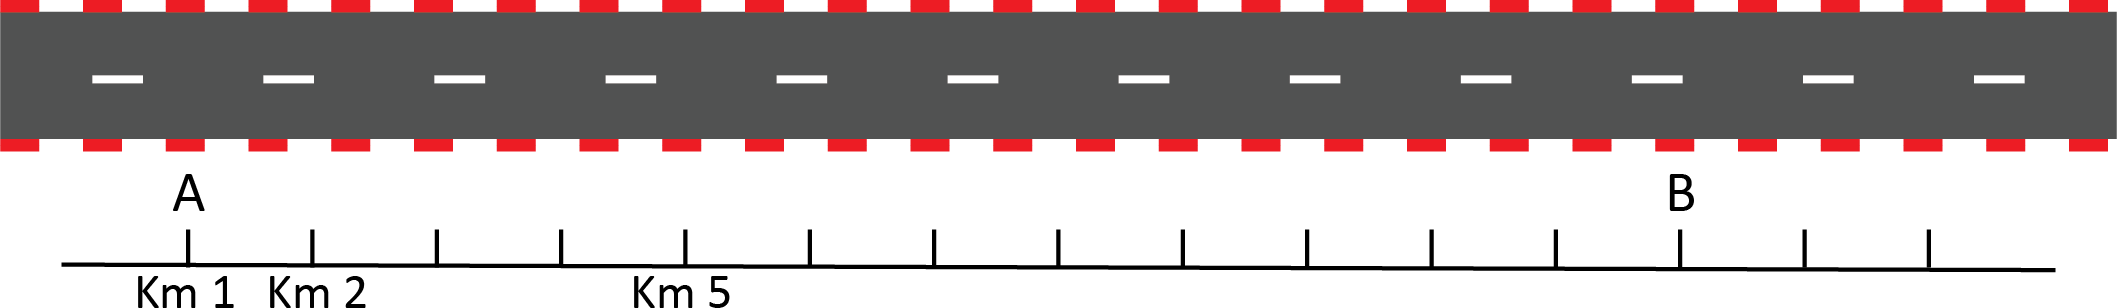
\includegraphics[width=\textwidth]{./media/image6.png}
\end{figure}

\vspace{1em}

Felipe desenhou uma linha reta para representar a distância de uma corrida de A até B. Ele também dividiu essa reta em intervalos de 1 km. 

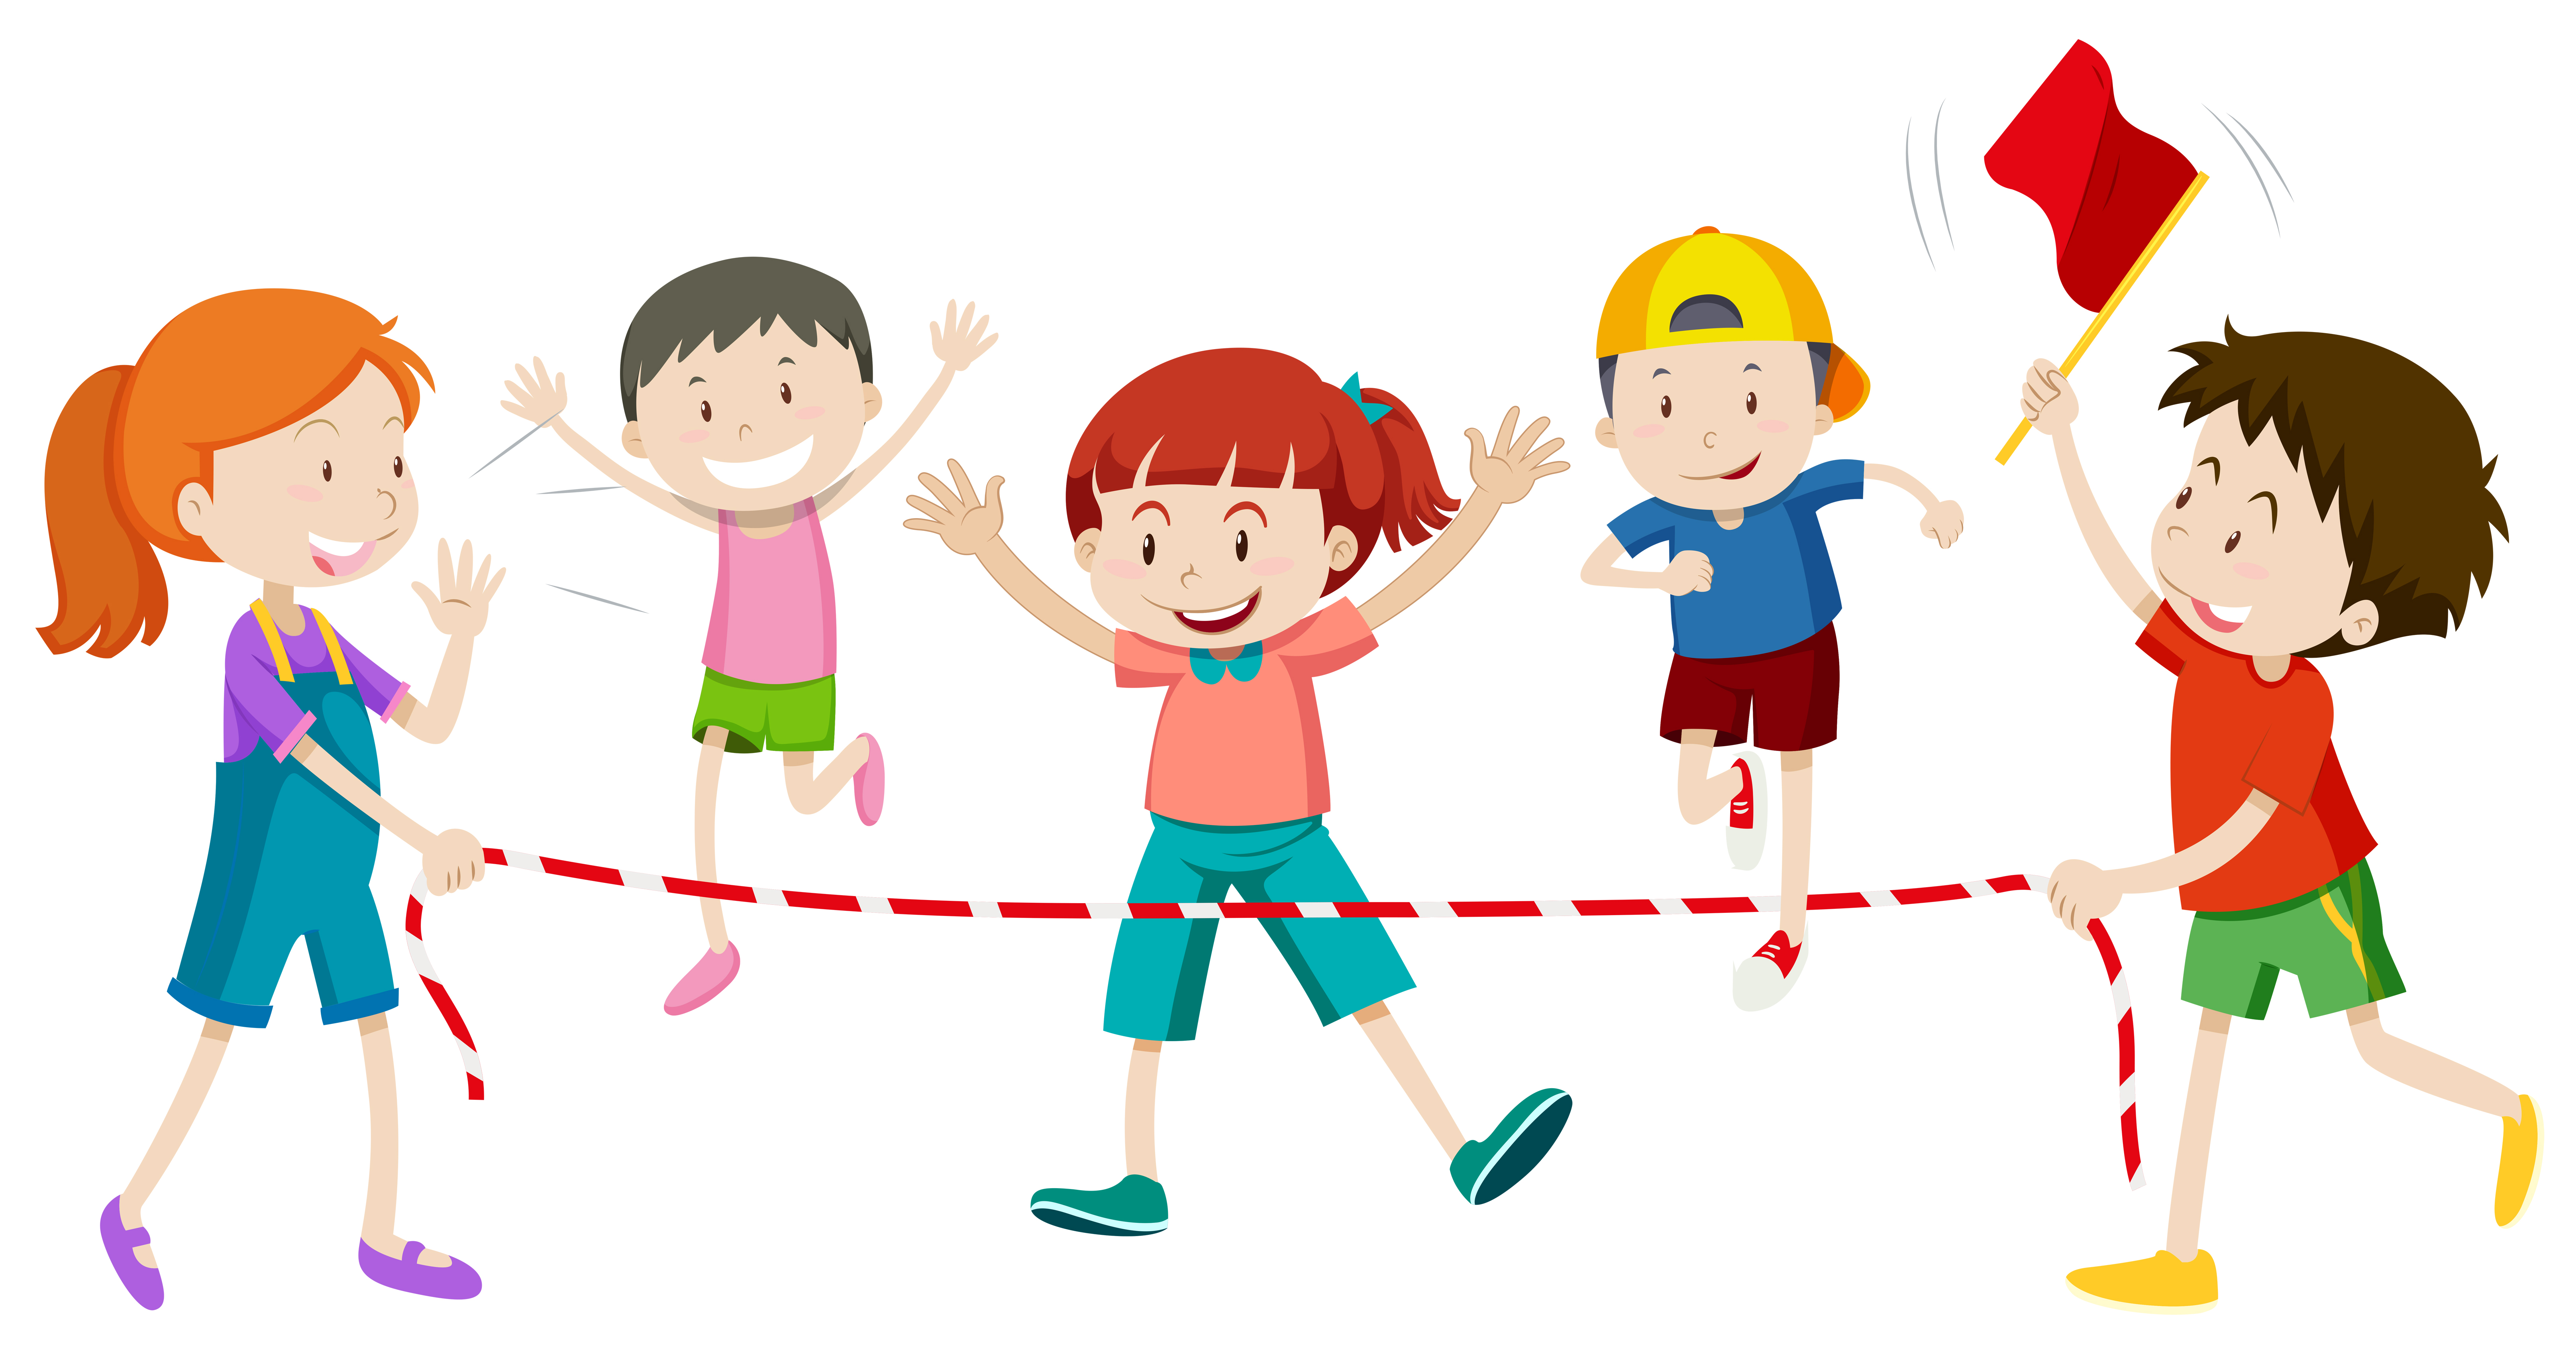
\includegraphics[width=\textwidth]{./media/image6a.jpeg}

\begin{escolha}
\item Calcule em que ponto Felipe parou na marcação, sabendo que ele completou a corrida.\\
\reduline{Km 12.\hfill}
\linhas{3}
\end{escolha}

\num{12} Ligue o número em algarismos da coluna 1 
à representação correspondente escrita por extenso na coluna 2.

\begin{figure}[htpb!]
\centering
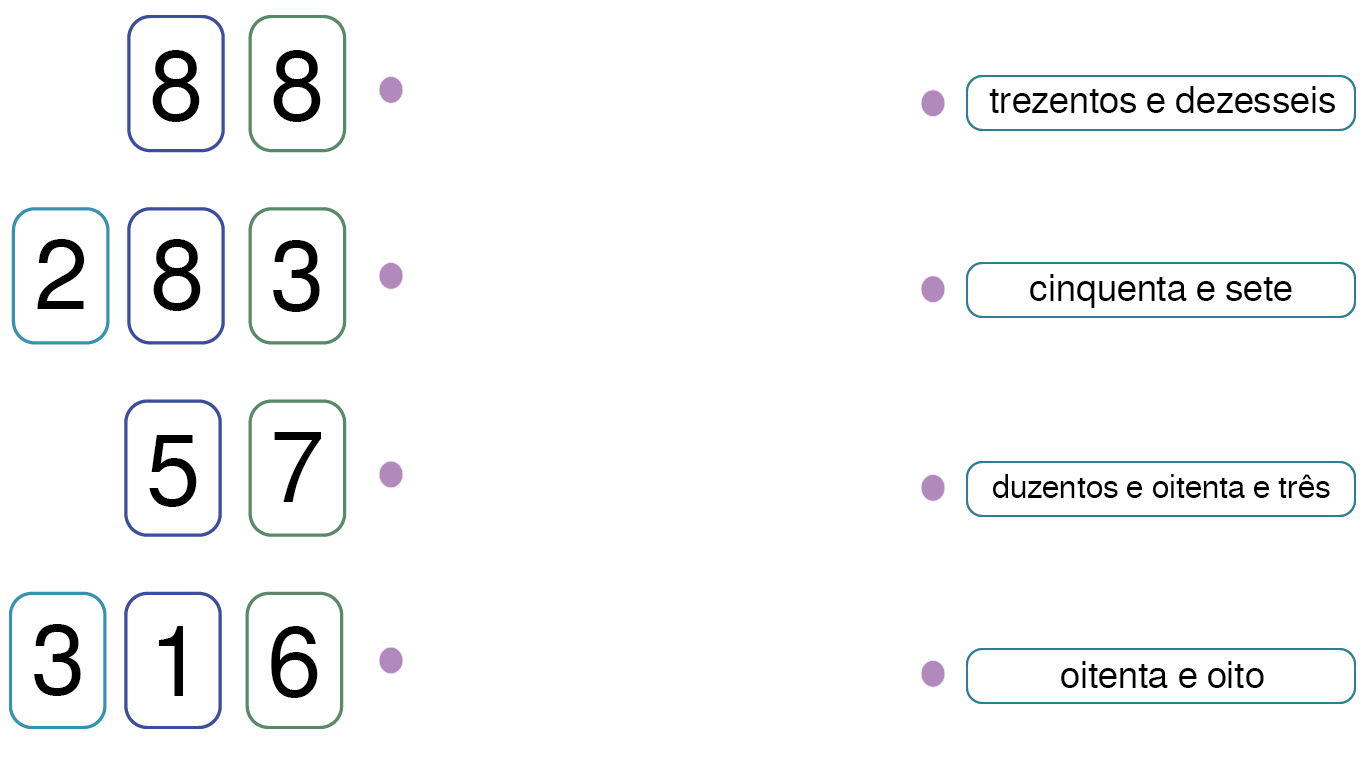
\includegraphics[width=\textwidth]{./media/image5.png}
\end{figure}

\coment{88 (oitenta e oito); 283 (duzentos e oitenta e três); 57 (ciquenta e sete); e 316 (a trezentos e dezesseis).}

%\sidetext{Felipe saiu do ponto A, que está em cima da marcação do quilômetro 0, e chegou ao
%ponto B, que está a 12 marcações de distância do ponto, podemos concluir
%que ele parou no km 12; ou seja, percorreu 12 km.

%Explore com os alunos a colocação dos números na reta numérica, considerando
%que é um conceito essencial em outros assuntos.}

\num{13} A bolas representadas na imagem abaixo fazem parte do jogo de sinuca. Observe os números e responda ao que se pede:

\begin{figure}[htpb!]
\centering
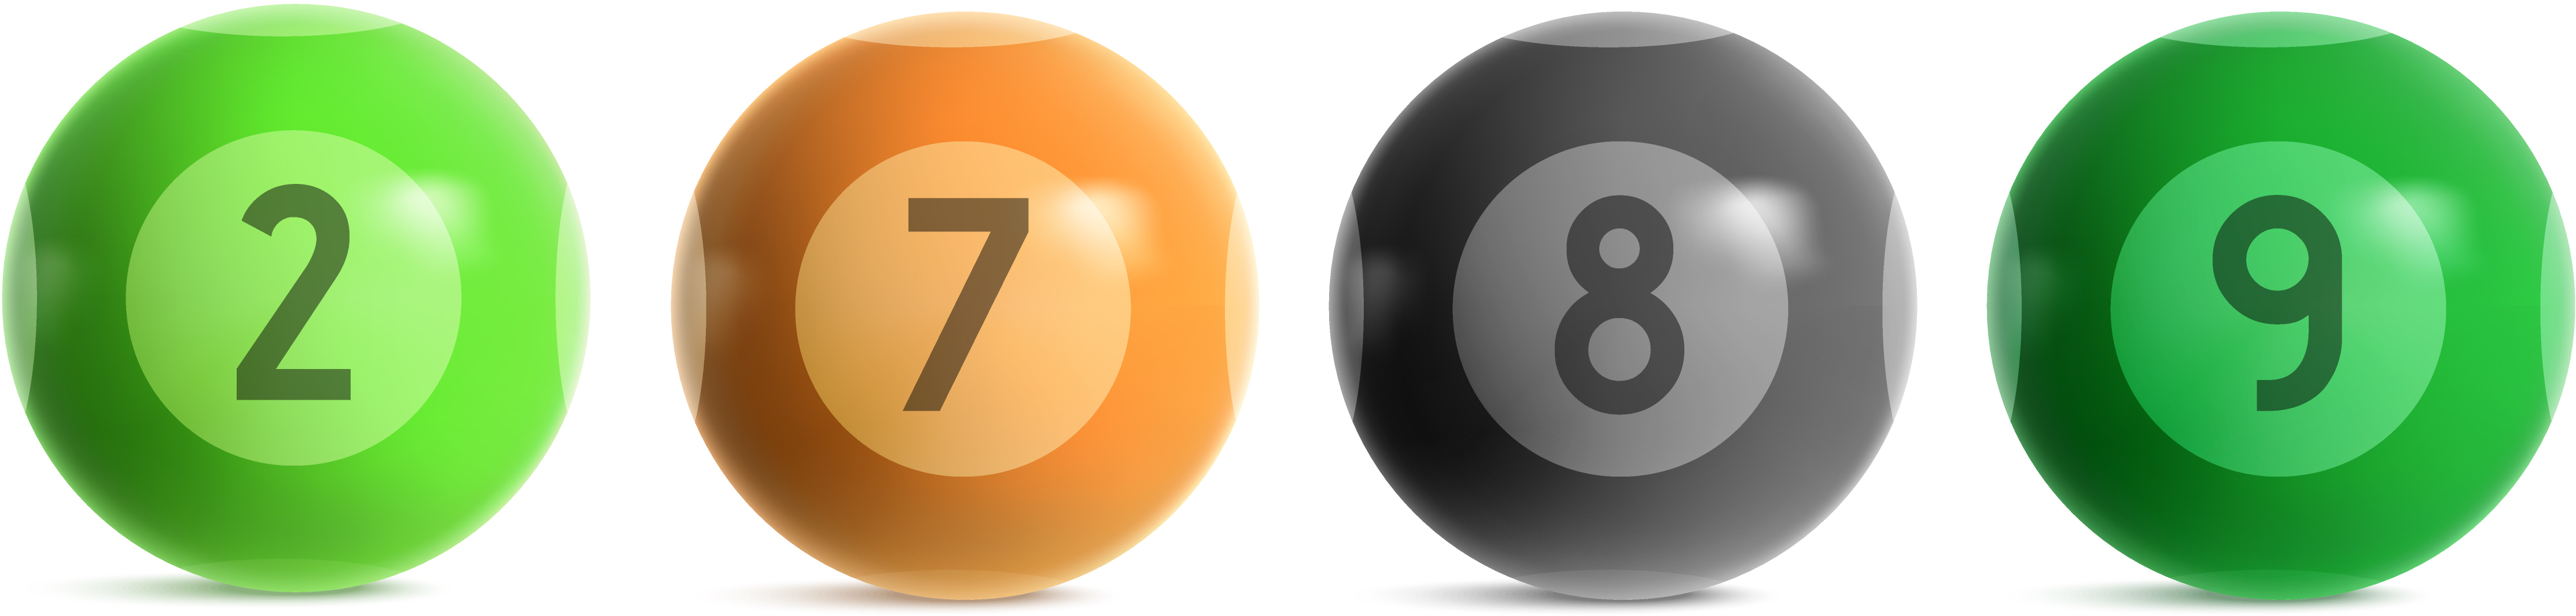
\includegraphics[width=.7\textwidth]{./media/image7.png}
\end{figure}

\begin{escolha}
\item Qual a bola de maior número?
\reduline{A bola de número é a de número 9 (nove).\hfill}

\item Usando os números das bolas, forme o menor número de três ordens. 
\reduline{O número é 278 (duzentos e setenta e oito).\hfill}

\item Usando os números das bolas, forme o maior número par.
\reduline{9.872 (nove mil oitocentos e setenta e dois).\hfill}

\end{escolha}

%\coment{Explore mais exemplos com os alunos para estimular a criatividade
%e a formação de números.}

\pagebreak

\section*{Treino}

\num{1} Amanda estava brincando no escritório de seu pai quando
encontrou um pedaço de papel com uma anotação: faturamento diário: 734 reais.

\begin{figure}[htpb!]
\centering

\includegraphics[width=0.6\textwidth]{./media/image6b.png}
\end{figure}

Lembrando-se das aulas de matemática, ela resolveu decompor o número escrito
no papel. Qual é a decomposição que Amanda deve fazer desse
número?

\begin{escolha}
\item
  700 + 30 + 4.
\item
  70 + 3 + 4.
\item
  700 + 40 + 3.
\item
  70 + 300 + 4.
\end{escolha}

\pagebreak

\num{2} Na reta numérica a seguir, o ponto P representa o número 540, e o ponto U representa o número 590.

\begin{figure}[htpb!]
\centering
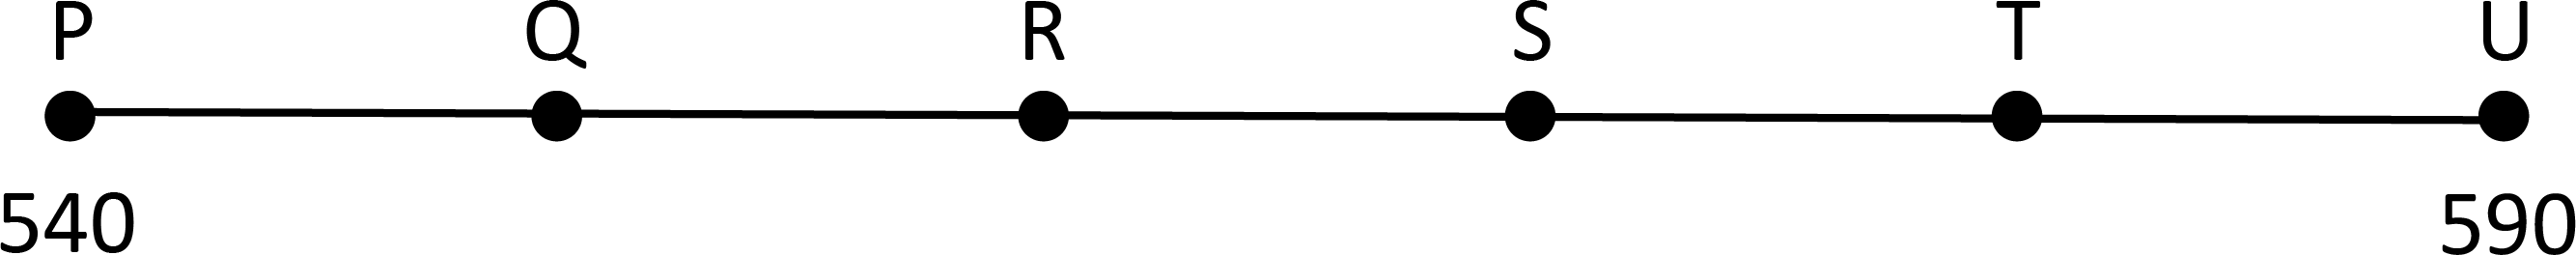
\includegraphics[width=\textwidth]{./media/image8.png}
\end{figure}

Indique o ponto correspondente à representação do número 570, sabendo que a
distância entre dois pontos consecutivos é de 10 unidades.

\begin{escolha}
  \begin{multicols}{2}
\item
  Q.
\item
  R.
\item
  S.
\item
  T.
  \end{multicols}
\end{escolha}

\num{3} Utilizando o material dourado, Ana Letícia montou um número.

\begin{figure}[htpb!]
\centering
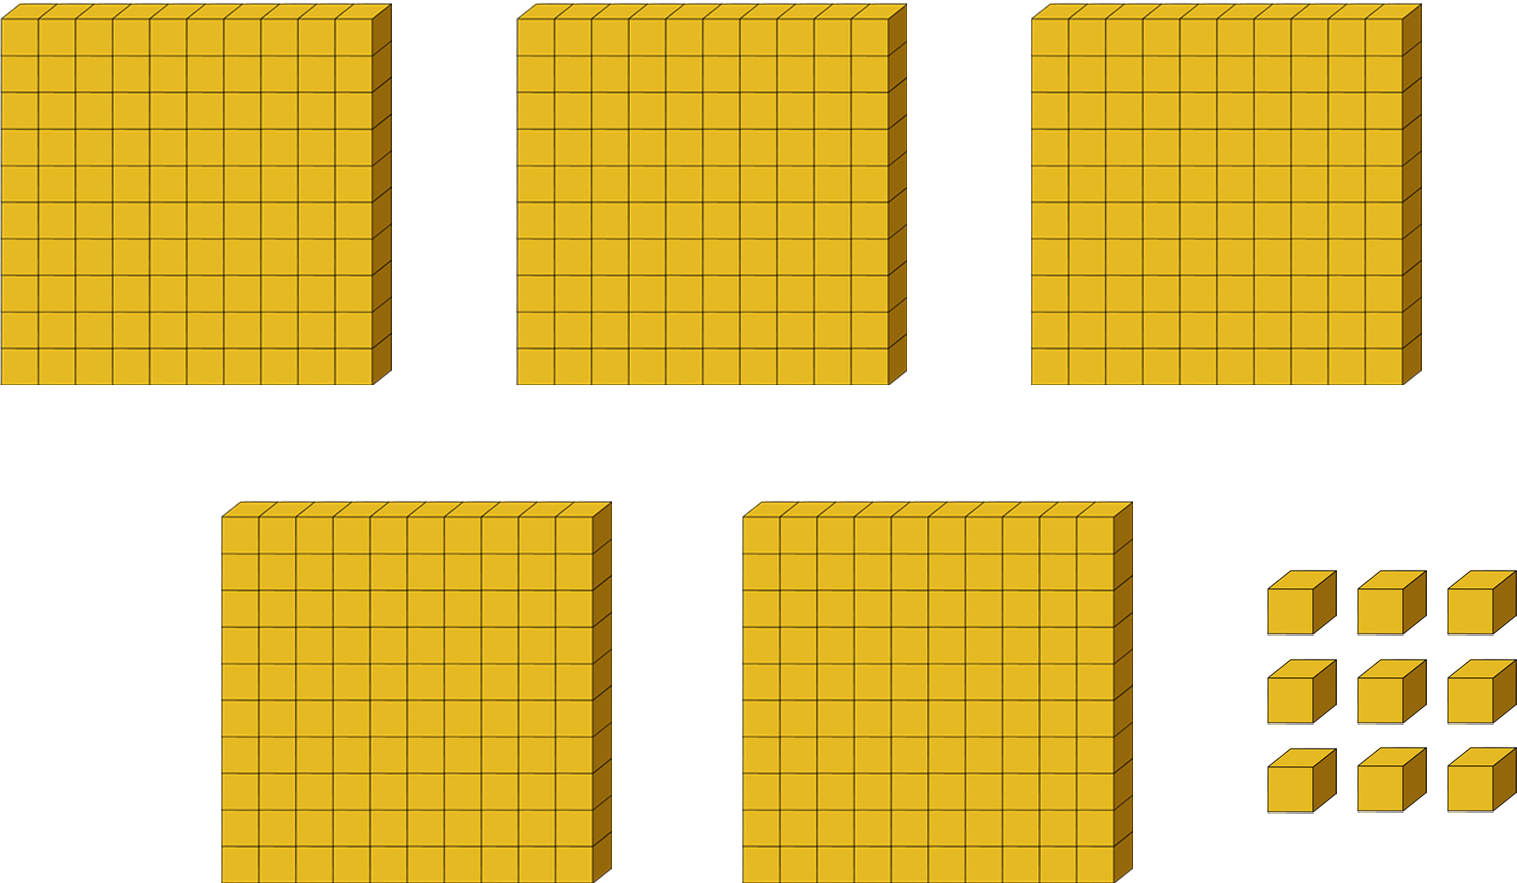
\includegraphics[width=\textwidth]{./media/image9.png}
\end{figure}

Qual é o número representado por Ana Letícia? 

\begin{escolha}
  \begin{multicols}{2}
\item
  59.
\item
  159.
\item
  509.
\item
  1.509.
  \end{multicols}
\end{escolha}

